The aim of this report is to investigate the abilities of autoencoder networks to reduce dimensionality and obtain meaningful representations from pretrained neural networks using images from the danish housing market.
This constitutes an unsupervised learning task, that is evaluated based on a models ability to produce dense representations that succeed in minimizing distance from similar images and increase distance to dissimilar images.
Throughout this report, key theoretical concepts relating to autoencoders and transfer learning are outlined and an extensive analysis of the appropriateness of autoencoders for this setting is conducted.
The focus of this report to conduct experiments in order to ascertain whether lower-cost methodologies can be leveraged to provide solutions in predicting image similarity on images of danish homes.

\subsection{The Domain Problem}
Individuals looking to find a house or an apartment of any sort in Denmark will inevitably rely on primitive aggregation sites, which allow them to filter based on some particular features for homes such as location, living area, price, etc.
According to \textbf{Danmarks Statistik}\footnote{Table: UDB010, https://rkr.statistikbank.dk/204}, between ~500-1000 new homes entered the market every month in the Copenhagen City Area and Frederiksberg alone in 2019 - that number is increasing.

This trend indicates that homeseekers will have to devote more time and effort in searching for a new home as they have no sophisticated tools at their disposal to do so. 
Homeseekers may also only periodically have the time to be alert on homes moving on and off the market and as such, they may not be aware that the perfect home has entered the market. 
\newline
It may also be the case, that homeseekers are actively looking regularly, using an aggregation service but are missing out on discovering suitable homes that do not match their filters. 
An example of this could be; a homeseeker has a strong preference for 1920's style apartments, enjoys large windows and open kitchens - also the homeseeker believes that the ideal apartment should be located in Frederiksberg and should be larger than $80m^{2}$.
This homeseeker may set up filters according to preferences wrt. size and location, but will have to sieve through many uninteresting prospects.
Furthermore, the homeseeker may be willing to consider a $79m^{2}$ apartment in an adjacent zip code, given that the aesthetic requirements are fulfilled.
The homeseeker will never be confronted with such homes.

\subsection{A Possible Solution}
Whilst the sale of fashion and lifestyle products has seen significant innovation with services like \textbf{Instagram} and \textbf{Pinterest}, many other industries are severely lacking behind. 
The technologies within image similarity put forward by e.g. \textbf{Pinterest}\autocite{Jing2015} suggest that consumers intuitively understand visual similarity for search purposes. 

\begin{figure}[H]
    \centering
    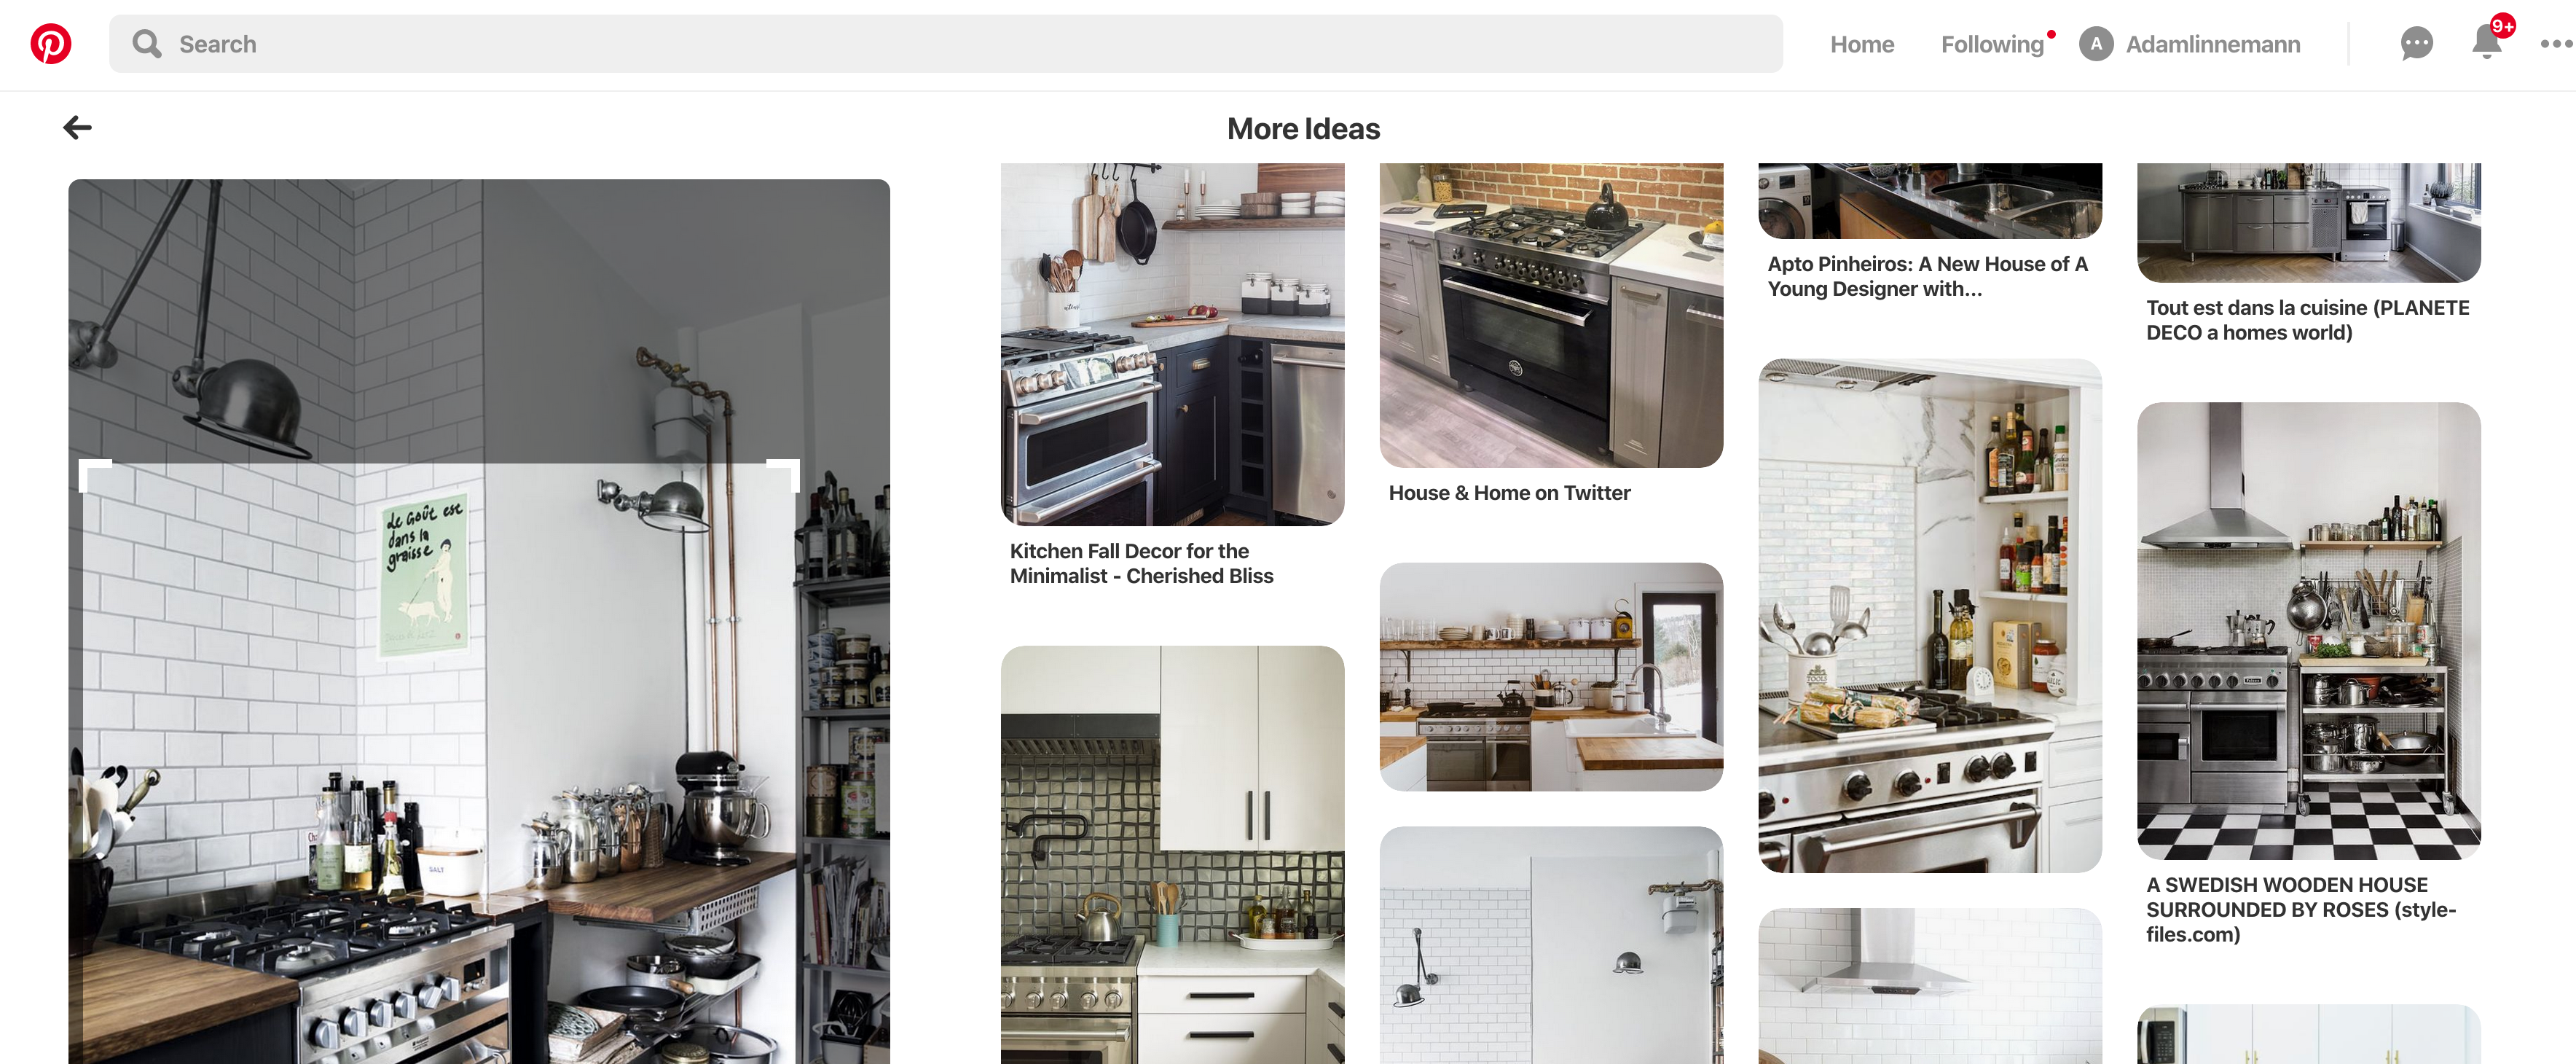
\includegraphics[scale=0.2]{pictures/random/pinterest1}
    \caption{Pinterest Visual Search}
    \label{ref:pinterest}
\end{figure}

Tools similar to those of \textbf{Pinterest} may aid homeseekers in:
\begin{enumerate}
    \item Filtering away homes that do not meet their aesthetic preferences
    \item Identifying homes that match their aesthetic preferences that they might not otherwise have found
\end{enumerate}

An improvement to the current services surrounding the danish real estate market may be to allow homeseekers to query for similar homes to ones they like based on visual similarity. 
Making it easier for homeseekers to identify e.g. 5 homes that suit their preferences wrt. aesthetics could be an aid to homeseekers and allow them to focus only on candidate homes that actually suit them, while casting a broader net wrt. size, location and other hard criteria.
\newline
The report will address the feasibility of visual search based on images from the danish real estate market.